\documentclass{ximera}
%herschreven 2 september 2026
\title{Het elektrisch veld van een puntlading}
\author{Daan Lipkens}

\begin{document}
\begin{abstract}
    De definitie van het elektrisch veld, testladingen en de veldsterkte van puntladingen.
\end{abstract}
\maketitle
% stuk rond hoe kracht staat bij negatieve test lading.
\section{Het concept van een elektrisch veld}

We zeggen dat er een \textbf{elektrisch veld} bestaat in de ruimte rondom een geladen voorwerp (de \textit{bronlading}). Wanneer een ander geladen voorwerp (de \textit{testlading}) in dit veld wordt geplaatst, zal het veld een elektrische kracht uitoefenen op deze testlading, zoals te zien op figuur~\ref{fig:testlading_bronlading}.

\begin{definition}[title={Het Elektrisch Veld}]\nl
    De elektrische veldvector $\vec{E}$ in een bepaald punt in de ruimte is gedefinieerd als de elektrische kracht $\vec{F}_e$ die inwerkt op een positieve testlading $Q_t$ in dat punt, gedeeld door de grootte van die testlading:
    $$ \vec{E} \equiv \frac{\vec{F}_e}{Q_t} $$
    De SI-eenheid van het elektrisch veld is de \textbf{newton per coulomb (N/C)}.
\end{definition}

%---------------------------
% AFBEELDING: Figuur 23.10 (Testlading bij bronlading)
\begin{figure}[ht!]
    \captionsetup{width=0.85\textwidth}
    \begin{center}
        
\includegraphics[height=8cm,width=12cm, keepaspectratio]{pic5/elektriciteit/veld/testlading_bronlading.png}
        % TIP: Gebruik hier de afbeelding van Figure 23.10 uit het boek
    \end{center}
    \caption{Een kleine positieve testlading $Q_t$ geplaatst in de buurt van een grotere positieve bronlading $Q$ ondervindt een elektrisch veld $\vec{E}$.}
    \label{fig:testlading_bronlading}
\end{figure}
%---------------------------

%---------------------------
% ANALOGIE ZWAARTEKRACHT
\begin{remark}[expandable, title={Analogie met het zwaarteveld}]\nl
    De definitie van het elektrisch veld lijkt heel sterk op iets wat we al kennen: het zwaarteveld! %Als veldkracht, een kracht dat geen contact nodig heeft om een invloed uit te oefenen, is er een bijhorend veld. Denk terug aan de zwaartekracht en het zwaarteveld.
    Net zoals een voorwerp met massa $m$ een zwaartekracht $\vec{F}_g$ ondervindt in het zwaarteveld $\vec{g}$ van de aarde, ondervindt een lading $Q_t$ een elektrische kracht $\vec{F}_e$ in een elektrisch veld $\vec{E}$.
    
    \begin{itemize}
        \item \textbf{Zwaarteveld:} $\vec{g} = \frac{\vec{F}_g}{m} \implies \vec{F}_g = m\cdot\vec{g}$
        \item \textbf{Elektrisch veld:} $\vec{E} = \frac{\vec{F}_e}{Q_t} \implies \vec{F}_e = Q_t\cdot\vec{E}$
    \end{itemize}

    \begin{center}
        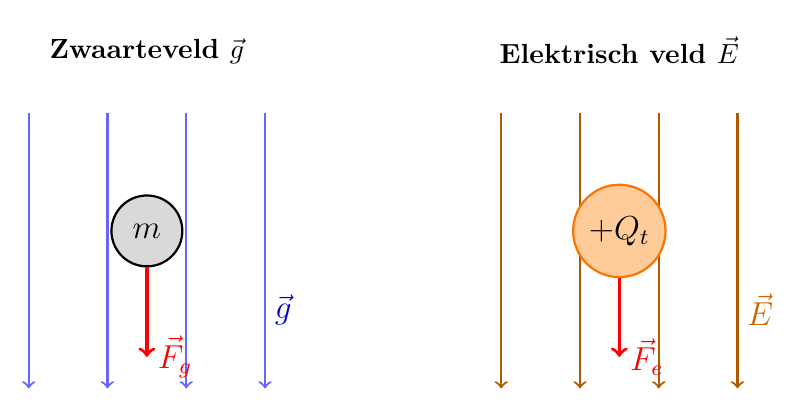
\begin{tikzpicture}[scale=1]
            % --- ZWAARTEVELD (Links) ---
            \node[above, font=\bfseries] at (0, 2) {Zwaarteveld $\vec{g}$};
            
            % Veldlijnen g (blauw)
            \foreach \x in {-1.5, -0.5, 0.5, 1.5} {
                \draw[->, thick, blue!60] (\x, 1.5) -- (\x, -2);
            }
            \node[blue!80!black, right, font=\large] at (1.5, -1) {$\vec{g}$};
            
            % Massa
            \node[circle, draw=black, fill=gray!30, thick, minimum size=9mm, font=\large] (m) at (0,0) {$m$};
            
            % Zwaartekracht
            \draw[->, very thick, red] (m) -- (0,-1.6) node[right, font=\large] {$\vec{F}_g$};

            % --- ELEKTRISCH VELD (Rechts) ---
            \node[above, font=\bfseries] at (6, 2) {Elektrisch veld $\vec{E}$};
            
            % Veldlijnen E (oranje)
            \foreach \x in {4.5, 5.5, 6.5, 7.5} {
                \draw[->, thick, orange!70!black] (\x, 1.5) -- (\x, -2);
            }
            \node[orange!80!black, right, font=\large] at (7.5, -1) {$\vec{E}$};
            
            % Lading
            \node[circle, draw=orange!90!red, fill=orange!40, thick, minimum size=9mm, font=\large] (q) at (6,0) {$+Q_t$};
            
            % Elektrische kracht
            \draw[->, very thick, red] (q) -- (6,-1.6) node[right, font=\large] {$\vec{F}_e$};
        \end{tikzpicture}
    \end{center}
\end{remark}
%---------------------------

\begin{proposition}[foldable=true,title={Eigenschappen van het elektrisch veld}]\nl
    \begin{itemize}
        \item Het veld $\vec{E}$ wordt gecreëerd door de bronlading(en), \textbf{niet} door de testlading zelf\footnote{De testlading zelf maakt ook een elektrisch veld, maar heeft geen invloed in dat punt zelf.}.
        \item Het veld bestaat in de ruimte rondom de bronlading, ongeacht of er effectief een testlading aanwezig is om het veld te detecteren.
        \item Als we de formule omvormen, kunnen we de kracht op elke willekeurige lading $Q$ in een gekend veld eenvoudig berekenen via $\vec{F}_e = Q\cdot \vec{E}$. Bij een positieve lading wijzen de kracht en het veld in dezelfde richting; bij een negatieve lading wijzen ze in tegengestelde zin.
    \end{itemize}
\end{proposition}


\begin{proposition}[foldable=true,title={Elektrische kracht op een lading in een elektrisch veld}]\nl
    De grootte van de kracht die op een lading $Q$ inwerkt in een elektrisch veld $E$ wordt gegeven door $F=Q\cdot E$. De richting van deze kracht is steeds evenwijdig met het elektrisch veld (zie figuur~\ref{fig:kracht_lading_in_veld}). De zin hangt af van het teken van de lading: bij een \textbf{positieve} lading heeft de kracht dezelfde zin als het elektrisch veld; bij een \textbf{negatieve} lading is de zin van de kracht net \textbf{tegengesteld} aan die van het elektrisch veld.
    %---------------------------------
% FIGUUR: kracht op lading in homogeen veld
\begin{center}
    \centering
    \begin{tikzpicture}[scale=1]
        % ----- PANEEL (a): positieve lading -----
        \begin{scope}
            % homogeen veld: evenwijdige veldlijnen naar rechts
            \foreach \y in {0, 1.2, 2.4}{
                \draw[vector] (0,\y) -- (3.4,\y);
            }
            \node[above] at (1.7,2.5) {$\vec{E}$};

            % lading tussen twee veldlijnen (geen overlap met de pijlen)
            \coordinate (Qpos) at (1.4,0.6);
            \draw[charge+] (Qpos) circle (2*\R) node[scale=1.3] {$+$};

            % kracht: zelfde zin als het veld
            \draw[force] (Qpos) ++ (2*\R+0.1,0) -- ++(1.1,0) node[right] {$\vec{F}$};

            \node[below] at (1.7,-0.5) {(a) positieve lading};
        \end{scope}

        % ----- PANEEL (b): negatieve lading -----
        \begin{scope}[xshift=6cm]
            \foreach \y in {0, 1.2, 2.4}{
                \draw[vector] (0,\y) -- (3.4,\y);
            }
            \node[above] at (1.7,2.5) {$\vec{E}$};

            \coordinate (Qneg) at (2.0,0.6);
            \draw[charge-] (Qneg) circle (2*\R) node[scale=1.3] {$-$};

            % kracht: tegengestelde zin aan het veld
            \draw[force] (Qneg) ++ (-2*\R-0.1,0) -- ++(-1.1,0) node[left] {$\vec{F}$};

            \node[below] at (1.7,-0.5) {(b) negatieve lading};
        \end{scope}
    \end{tikzpicture}
    \captionof{figure}{De kracht op een lading in een homogeen elektrisch veld. (a) Op een positieve lading werkt de kracht in dezelfde zin als het veld. (b) Op een negatieve lading werkt de kracht in de tegengestelde zin.}
    \label{fig:kracht_lading_in_veld}
\end{center}
%---------------------------------

\end{proposition}


\section{Elektrisch veld van een puntlading}
\subsection{Formule elektrisch veld van een puntlading}

We kunnen de grootte van het elektrisch veld van één enkele puntlading afleiden door de wet van Coulomb in onze velddefinitie te stoppen. De kracht die bronlading $Q_b$ uitoefent op testlading $Q_t$ op afstand $r$ is:
$$ F_e = k_e \frac{|Q_b| \cdot |Q_t|}{r^2} $$

Als we dit delen door $Q_t$, bekomen we de grootte van het elektrisch veld veroorzaakt door $Q_b$:

\begin{definition}[title={Formule radiaal veld}]\nl
    $$E = k_e \frac{|Q_b|}{r^2}$$
\end{definition}

\begin{proposition}[foldable=true,title={De \textbf{richting en zin} van het elektrisch veld}]\nl
    \begin{itemize}
        \item Is de bronlading \textbf{positief}, dan wijst de veldvector \textbf{radiaal weg}\footnote{Het elektrisch veld van een puntlading wordt een radiaal veld genoemd, zie sectie \ref{s:radiaalveld}.} van de lading (omdat een positieve testlading zou worden afgestoten).
        \item Is de bronlading \textbf{negatief}, dan wijst de veldvector \textbf{radiaal naar de lading toe} (omdat een positieve testlading zou worden aangetrokken).
    \end{itemize}

    %---------------------------
    % AFBEELDING: Figuur 23.11 (Veldvectoren rond puntlading)
    \begin{center}
        \captionsetup{width=0.85\textwidth}
        
\includegraphics[height=10cm,width=14cm,keepaspectratio]{pic5/elektriciteit/veld/veld_puntlading.png}
        % TIP: Gebruik hier Figure 23.11 uit het boek (a, b, c, d)
        \captionof{figure}{Een testlading $q_0$ in punt \textit{P} bevindt zich op een afstand $r$ van een puntlading $q$. (a) Als $q$ positief is, is de kracht op de testlading weg van $q$ gericht. (b) Bij een positieve bronlading wijst het elektrisch veld in \textit{P} radiaal weg van $q$. (c) Als $q$ negatief is, is de kracht op de testlading naar $q$ toe gericht. (d) Bij een negatieve bronlading wijst het elektrisch veld in \textit{P} radiaal naar $q$ toe.}
        \label{fig:veld_puntlading}
    \end{center}
    %---------------------------
\end{proposition}

%———————————————————————————————————————
% VRAAG: Quick Quiz 23.4
\begin{question}
    Een positieve testlading van $+3{,}0 \, \mu\mathrm{C}$ wordt geplaatst in punt \textit{P} in de ruimte. Deze ondervindt een extern elektrisch veld dat naar rechts is gericht met een grootte van $4{,}0 \cdot 10^{6} \, \mathrm{N/C}$. Stel dat we deze testlading weghalen, en vervangen door een nieuwe testlading van $-3{,}0 \, \mu\mathrm{C}$. Wat gebeurt er dan met het externe elektrisch veld in punt \textit{P}?

    \begin{multipleChoice}
        \choice[correct]{Het veld blijft ongewijzigd.}
        \choice{De richting van het veld draait om.}
        \choice{Het verandert op een onvoorspelbare manier.}
    \end{multipleChoice}

    \begin{hint}
        Wordt een elektrisch veld opgewekt door de bronlading(en) of door de testlading?
    \end{hint}

    \begin{solution}\nl
        Het externe elektrische veld wordt gegenereerd door (niet-weergegeven) bronladingen, niet door de testlading zelf. Het weghalen of veranderen van een testlading heeft geen enkele invloed op het veld dat er al aanwezig was. De \textit{kracht} op de testlading zal natuurlijk wel van richting veranderen, maar het \textit{veld} niet!
    \end{solution}
\end{question}
%———————————————————————————————————————

\subsection{Superpositiebeginsel}
Wanneer er meerdere puntladingen aanwezig zijn, bereken je het totale elektrisch veld in een willekeurig punt \textit{P} door de veldvectoren van elke bronlading afzonderlijk te berekenen, en deze vervolgens \textbf{vectorieel op te tellen}\footnote{Zie bijlage \ref{s:vectoren_optellen}.}.

$$ \vec{E}_{tot} = \vec{E}_1 + \vec{E}_2 + \vec{E}_3 + \dots $$

Wanneer de bronladingen zich op één rechte lijn bevinden, samen met het punt \textit{P} waar we het veld willen kennen, vereenvoudigt deze vectoriële optelling tot een gewone algebraïsche optelling: we kiezen een positieve zin langs de lijn en tellen de (positieve of negatieve) bijdragen van elke bronlading gewoon bij elkaar op.

%---------------------------
% VOORBEELD: superpositie op een lijn
\begin{example}[foldable=true,title={Superpositie van twee puntladingen op een lijn}]\nl
    Twee puntladingen bevinden zich op de $x$-as: $Q_{1}=+5{,}0 \cdot 10^{-6} \, \mathrm{C}$ bij $x=0{,}00 \, \mathrm{m}$ en $Q_{2}=-2{,}0 \cdot 10^{-6} \, \mathrm{C}$ bij $x=0{,}40 \, \mathrm{m}$. Bereken het resulterende elektrisch veld in punt $P$ op $x=0{,}60 \, \mathrm{m}$.
    \begin{solution}\nl
        We berekenen eerst de grootte van elk afzonderlijk veld met de formule voor het radiaal veld van een puntlading.

        Veld van $Q_{1}$ in $P$ (afstand $r_{1}=0{,}60 \, \mathrm{m}$):
        \[
            E_{1}=k_{e}\frac{|Q_{1}|}{r_{1}^{2}}=\frac{8{,}99 \cdot 10^{9} \, \mathrm{\frac{N \cdot m^2}{C^2}} \cdot 5{,}0 \cdot 10^{-6} \, \mathrm{C}}{(0{,}60 \, \mathrm{m})^{2}}=1{,}2 \cdot 10^{5} \, \mathrm{N/C}
        \]
        Omdat $Q_{1}$ positief is, wijst $\vec{E}_{1}$ in $P$ weg van $Q_{1}$: naar rechts (de $+x$-richting).

        Veld van $Q_{2}$ in $P$ (afstand $r_{2}=0{,}20 \, \mathrm{m}$):
        \[
            E_{2}=k_{e}\frac{|Q_{2}|}{r_{2}^{2}}=\frac{8{,}99 \cdot 10^{9} \, \mathrm{\frac{N \cdot m^2}{C^2}} \cdot 2{,}0 \cdot 10^{-6} \, \mathrm{C}}{(0{,}20 \, \mathrm{m})^{2}}=4{,}5 \cdot 10^{5} \, \mathrm{N/C}
        \]
        Omdat $Q_{2}$ negatief is, wijst $\vec{E}_{2}$ in $P$ naar $Q_{2}$ toe: naar links (de $-x$-richting).

        Beide velden liggen op dezelfde lijn, dus tellen we ze algebraïsch op (rechts is positief):
        \[
            E_{\text{net}}=E_{1}-E_{2}=1{,}2 \cdot 10^{5} \, \mathrm{N/C} - 4{,}5 \cdot 10^{5} \, \mathrm{N/C} = -3{,}2 \cdot 10^{5} \, \mathrm{N/C}
        \]
        Het resulterende veld heeft een grootte van $3{,}2 \cdot 10^{5} \, \mathrm{N/C}$ en wijst naar links (de $-x$-richting), dus naar de ladingen toe.
    \end{solution}
\end{example}
%---------------------------

\end{document}